\section{Computation of the Mandelbrot Set}

\begin{figure}[tb]
  \centering
  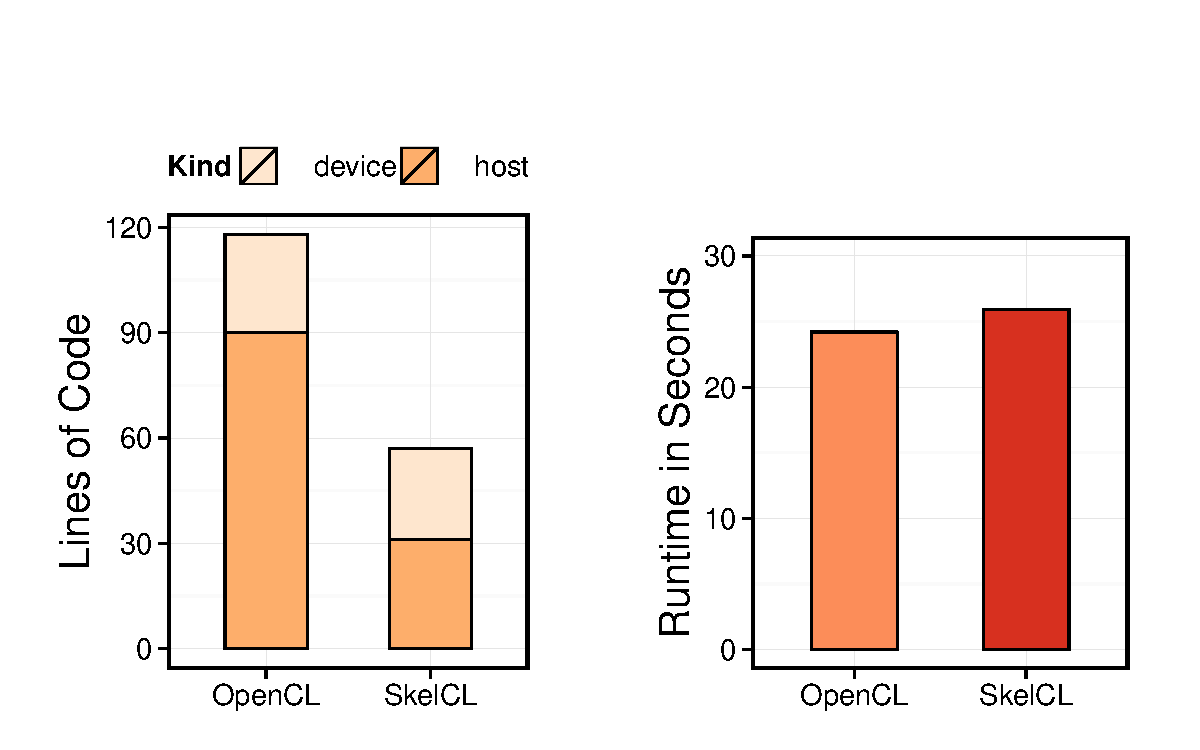
\includegraphics[width=.75\textwidth]{mandelbrot}
  \caption{Visualization of a part of the Mandelbrot set. The image was produced using the \SkelCL library.}
  \label{fig:mandelbrot}
\end{figure}

The Mandelbrot~\cite{Mandelbrot1980} set are all complex numbers $c \in {\mathbb C}$ for which the sequence
\begin{equation}
	z_{i+1} = z_{i}^{2} + c,\qquad i\in {\mathbb N}
	\label{eq:mandelbrot}
\end{equation}
starting with $z_{0}=0$ does not escape to infinity.
When drawn as an image with each pixel representing a complex number, the boundary of the Mandelbrot set forms a fractal.
\autoref{fig:mandelbrot} shows a part of an image visualizing the Mandelbrot set.
The software producing the image was implemented using the \SkelCL library. 
The calculation of such an image is a time-consuming task, because the sequence given by~\autoref{eq:mandelbrot} has to be calculated for every pixel.
If this sequence does not cross a given threshold for a given number of steps, it is presumed that the sequence will converge.
The respective pixel is thus taken as a member of the Mandelbrot set, and it is displayed black.
Other pixels outside are assigned a color that corresponds to the number of iterations of the sequence given by~\autoref{eq:mandelbrot}.
Computing a Mandelbrot fractal is easily parallelizable, as all pixels of the fractal can be computed simultaneously.

We created three similar parallel implementations for computing a Mandelbrot fractal using CUDA, OpenCL, and \SkelCL.
We compare the programming effort and performance for these implementations.

\subsubsection{Programming effort}
\label{sec:mandelbrot:implementation}

CUDA and \SkelCL require a single line of code for initialization in the host code, whereas OpenCL requires a lengthy creation and initialization of different data structures which take about 20 lines of code.

The host code differs significantly between all implementations.
In CUDA, the kernel is called like an ordinary function.
A proprietary syntax is used to specify the size of work-groups executing the kernel.
With OpenCL, several API functions are called to load and build the kernel, pass arguments to it and to launch it using a specified work group size.
In \SkelCL, the \map skeleton is used to compute the color of all pixels in the image.
A \code{Matrix} of complex numbers, each of which is represented by a pixel of the Mandelbrot fractal, is passed to the \map skeleton upon execution.
Specifying the work group size is mandatory in CUDA and OpenCL, whereas this is optional in \SkelCL.

\paragraph{Program size}
The OpenCL-based implementation has 118 lines of code (kernel: 28~lines, host program: 90~lines) and is thus more than twice as long as the CUDA and \SkelCL versions with 49 lines (28, 21) and 57 lines (26, 31), respectively (see \autoref{fig:mandelbrot_runtime}).
The length of the CUDA- and \SkelCL-based implementations differs by only a few lines.

\paragraph{Kernel size}
The kernel function is similar in all implementations: it takes a pixel's position (\ie, a complex number) as input, performs the iterative calculation for this pixel, and returns the pixel's color.
However, while the input positions are given explicitly when using the \map skeleton in SkelCL, no positions are passed to the kernel in the CUDA- and OpenCL-based implementations.
The positions are implicitly determined based on the work item's index.

\subsubsection{Performance experiments}
\label{sec:mandelbrot:runtime}

\begin{figure}[tb]
    \centering
    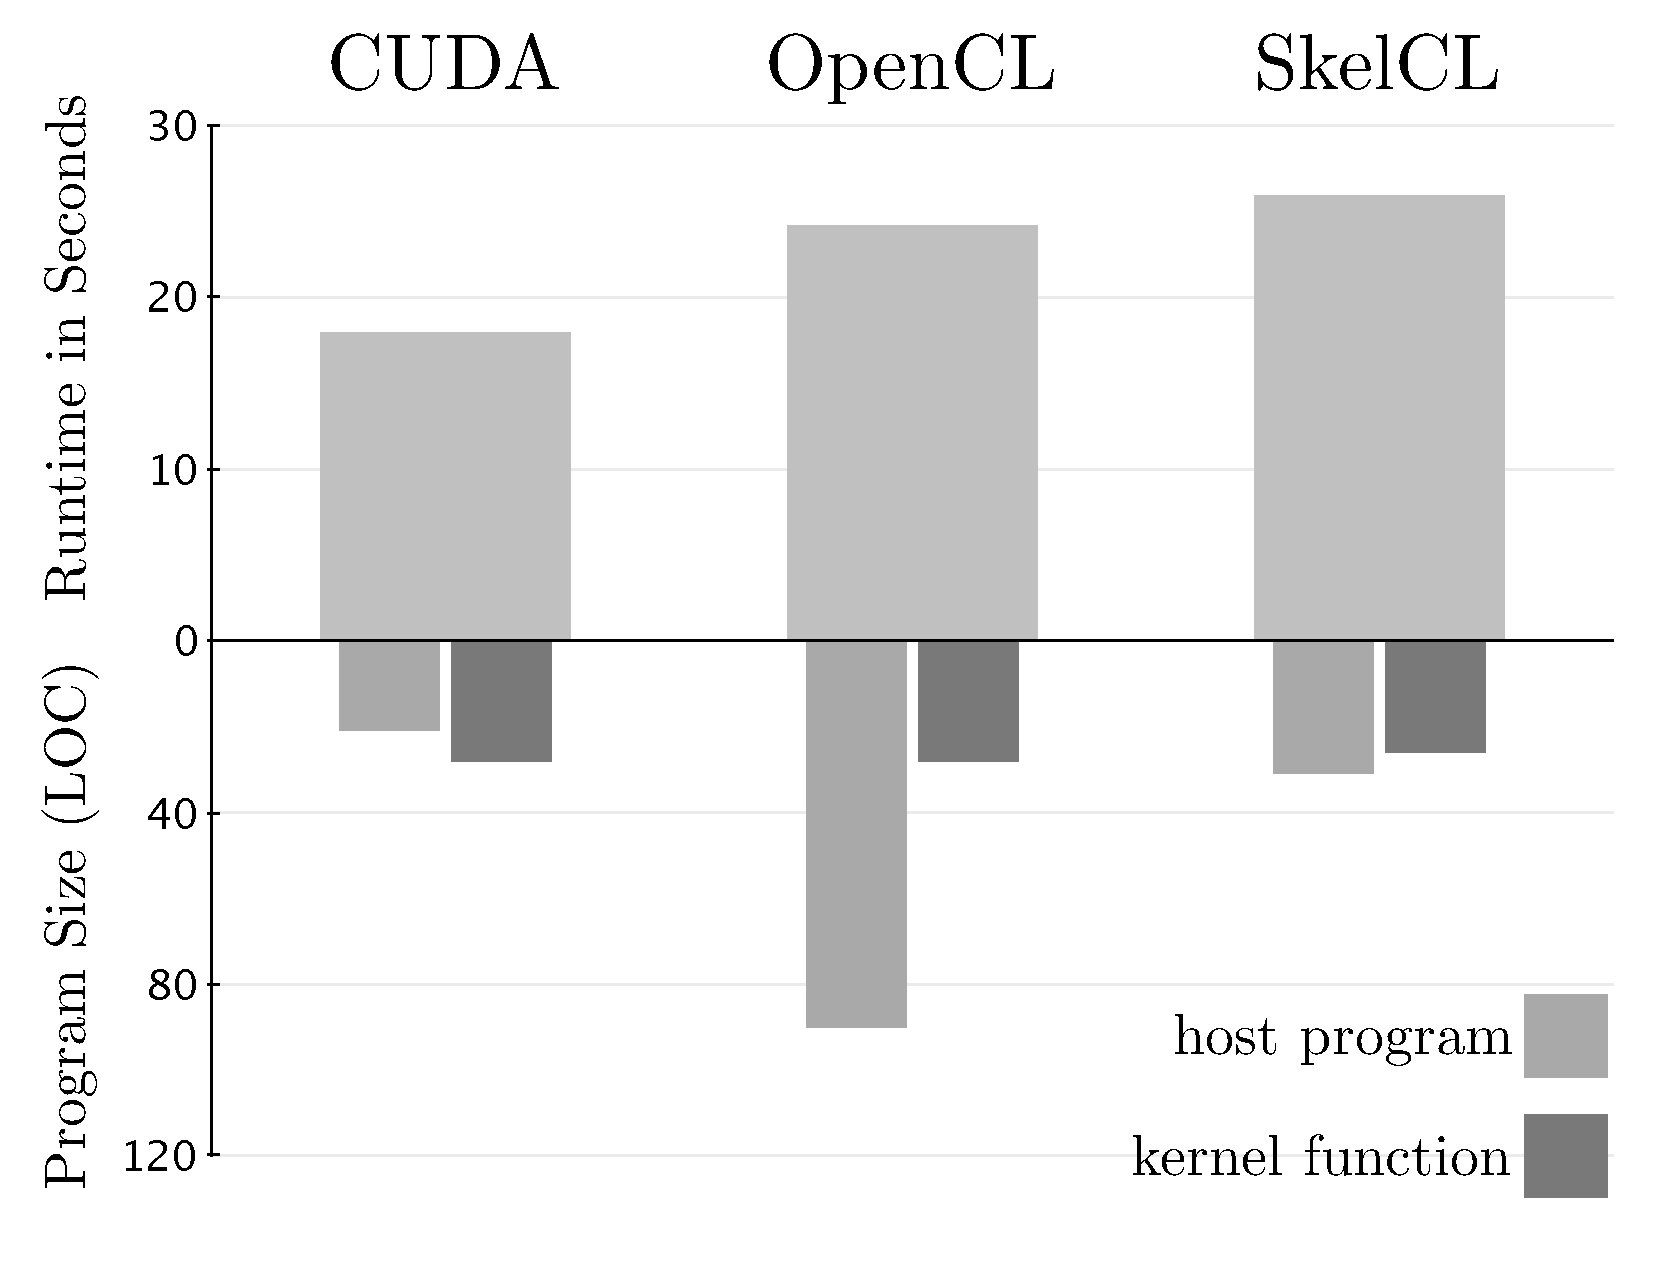
\includegraphics[width=0.6\textwidth]{HIPS/ChartMandelbrot}
    \caption{Runtime and program size of the Mandelbrot application.}
    \label{fig:mandelbrot_runtime}
\end{figure}%


We tested our implementations on a single \GPU of our test system to compute a Mandelbrot fractal of size 4096$\times$3072 pixels.
In CUDA and OpenCL, work groups of 16$\times$16 are used; \SkelCL uses its default work group size of~256 work items.
The results are shown in \autoref{fig:mandelbrot_runtime}.
As compared to the runtime of the \SkelCL-based implementation (26 seconds), the implementation based on OpenCL (25 seconds) and CUDA (18 seconds) are faster by 4\% or 31\%, respectively.
Since \SkelCL is built on top of OpenCL, the performance difference of \SkelCL and OpenCL can be regarded as the overhead introduced by SkelCL.
Previous work~\cite{KongDiYaLiCaStMaZh2010} also reported that CUDA was usually faster than OpenCL, which also explains the higher performance of the implementation based on CUDA.
The Mandelbrot application demonstrates that \SkelCL introduces a tolerable overhead of less than 5\% as compared to OpenCL.
A clear benefit of this overhead is the reduced programming effort required by the SkelCL program.

